\textbf{Notes}

\begin{enumerate}
    \item GLSL preloading processors as implemented by me
    \item Rounding errors in GLSL vs Python (x >= 0.05 == false in GLSL but x >= 0.05 == true in python).
    \item What has been done to minimize mistakes in python translation between openGL and python?
    \begin{enumerate}
        \item Naming
        \item array -> vec3
        \item frag color returned
        \item division adds TINY\_FLOAT
    \end{enumerate}
    \item How to handle negative colors?
    \item \st{Explain about the convention of column major? }
    \item \st{Explain why we use 3 channels (why the alpha value is omitted)}
\end{enumerate}

\section{Forward Rendering in OpenGL}\label{sec:RenderingInOpenGL}
\textbf{Why is this section here? How is it used in DiPTeR?}

\subsection{Rendering Pipeline}

\begin{figure}[!h]
    \centering
    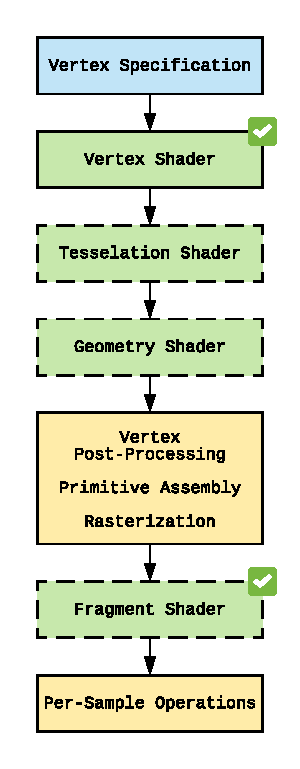
\includegraphics{img/theory/RenderingPipeline.pdf}
    \caption{An overview of the different stages in the OpenGL Rendering Pipeline. The stage marked blue is not programmable, but still defined by the user. The stages marked yellow are not controllable by the user. The stages marked green are programmable by user-defined shaders, where the dashed outline marks optional stages. A checkmark icon marks the only stages that are used in this project.}
    \label{fig:RenderingPipeline}
\end{figure}

The OpenGL rendering pipeline consists of multiple different stages, defining a workflow starting with 3D vertex data to finally producing 2D pixels on a screen \cite{a2019_rendering}. Some of these stages are programmable by the user, marked in green, in figure \ref{fig:RenderingPipeline}, while the Vertex Shader is the only one that is \textit{required} to be defined by the user. A shader is a program typically written in the GLSL language that takes a specific type of input, processes it, and outputs a specific type and is designed to run on a particular stage in the pipeline. The shaders has a pre-defined minimum amount of input, but can also take user-defined input.

In the Vertex Specification step, no shader is used, but a list of vertex positions is defined to be rendered as well as a list of triangles that define the faces between these vertices. The Vertex Shader is run on each of these vertices and takes exactly one vertex as input and outputs exactly one vertex. This shader typically also takes three transformation matrices as input that define the scaling, translation and rotation of the object. These are used to output vertices in \textit{clip space}, see section \ref{sec:CoordinateSystem}. Next up is the Tesselation Shader and the Geometry Shader. Both manipulate or create geometry but neither are used in our project, as we are only interested in the look of the objects texture, not its geometry. Before the Fragment Shader stage, there is a crucial \textit{rasterization} stage that needs to be completed. This stage turns primitives (like triangles) into fragments, by looping over screen pixels and checking if they lie inside the boundaries of a primitive. If they do, a fragment is created for this pixel and the fragment is given per-vertex values that are interpolated between the vertices that make up the primitive, see section \ref{sec:Interpolation}. The fragments are closely related to screen pixels, but contain more information and each pixel can spawn more than one fragment, depending on multisampling parameters. Each fragment is then sent, one by one, to a Fragment Shader (also called Pixel Shader) which is where all the computations are done that define the final color of a single fragment. In essence, a fragment shader defines a function $f(V,P) \mapsto (r,g,b,a)$ that takes a set of interpolated per-vertex parameters $V$ and a set of user defined parameters $P$ as input, and outputs a fragment color on the form $(r,g,b,a)$, where $r$, $g$, $b$ are the value of the red,green and blue channels, respectively and $a$ is the alpha value of the fragment.

\subsection{Coordinate Systems}\label{sec:CoordinateSystem}

\textbf{IMAGE EXPLAINING THE DIFFERENT SPACES!} \href{https://learnopengl.com/Getting-started/Coordinate-Systems}{SOURCE}

In OpenGL there are five different coordinate spaces of interest, and three different transformation matrices that are used to convert between them. The first, \textit{object space}, is the space that is local to a 3D object in the scene. The axes of the local object space are static in relation to the object, no matter how the object is rotated, translated or scaled. As a comparison, a persons left and right will always be the same in relation to that person, but different when compared to another person because it is local to that person. To be able to position object relative to each other, we define a world space. Again, using a real world comparison, this corresponds to the cardinal directions of earth. Moving two objects north on global space, even with different individual local rotations, would move them along the global y-axis. To convert object coordinates to global coordinates, they are multiplied with a matrix often referred to as the \textit{object-to-world} matrix. In OpenGL, we do not need to render everything in the 3D scene, but only what is seen from a camera or viewer's point of view. As such, this space is referred to as view space or camera space. Coordinates in world space are converted to view space with a matrix conveniently referred to as the \textit{world-to-view} matrix. The object are now in a coordinate space that makes sense to the user. Moving an object left to right in view space (along x-axis) will move it left to right on the screen. However, as an OpenGL convention, any vertices outside of the range $[-1,1]$ will be \textit{clipped} or discarded and thus not rendered. Therefore, the next space is referred to as clip space and the coordinates in the range $[-1,1]$ as \textit{Normalized Device Coordinates} or NDC. A user can either define all of its vertices as NDC or in an arbitrary coordinate system and normalize them at this stage. The coordinates are converted from world space to clip space using a \textit{view-to-projection} matrix as the process of converting user defined coordinates to NDC (that are easy to map to a two dimensional coordinate system) is called \textit{projection}. This matrix comes in two forms, depending if \textit{perspective} or \textit{orthographic} projection is used.

Using the three matrices, it's straight forward to attain the final NDCs in clip space by multiplying the vertices in user defined coordinates with each matrix as seen in equation \ref{eq:ObjectToClipCoordinates}. This defines the required output of the vertex shader, but there is one last important coordinate space to be aware of. This process is called the \textit{viewport transform} and converts the NDCs to screen coordinates, so that each point is mapped to a pixel on the screen. This coordinate system has its origin in the lower left corner of the screen at position $(0,0)$ and runs up to the defined resolution for the OpenGL viewport \textbf{IMAGE SHOWING THIS?}.

\begin{equation}\label{eq:ObjectToClipCoordinates}
    V_{clip} = M_{view-to-projection} \cdot M_{world-to-view} \cdot M_{object-to-view} \cdot V_{user}
\end{equation}

\subsection{Interpolation}\label{sec:Interpolation}
\begin{enumerate}
    \item[\done] How per-vertex attributes gets interpolated to frag shader (frag\_pos) or color
    \item[\done] How the vertex positions are samples (middle of interval)!
    \item[\done] PROVIDE IMAGE OF frag\_pos being interpolated!
    \item Should the bit about half-pixel position be moved to coordinate system?
\end{enumerate}

Any input attributes to the fragment shader (declared using the \codeinline[glsl]{in} keyword) is interpolated between vertices before being sent to the fragment shader. Its important to notice that vertices may not only contain a position, but other arbitrary data referred to as \textit{attributes}, which also gets interpolated. In this way, its possible to provide the fragment shader with normalized fragment positions as long as the position is set in the vertex shader. This special variable is extensively used in our shaders and will be referred to as  \codeinline[python]{frag_pos} and is a vector on the form $(x,y,z)$ where $x,y,z \in [0,1]$. Having a normalized fragment position means that no matter how our object is shaped, every position on its surface is defined in the range $[0,1]$ where a value of $1.0$ identifies the maximum point on that object in a specific direction. As explained in section \ref{sec:CoordinateSystem}, a user can define the vertices in any arbitrary coordinate system, as long as they are normalized in the vertex shader. To do this, the maximum and minimum value of the user defined coordinate system is needed as input to the vertex shader. The attribute \codeinline[glsl]{frag_pos} is calculated as $frag\_pos = \frac{in\_vert\_pos - mins}{maxes-mins}$. After the rasterizer has calculated which fragments belong to which triangle, the vertex attributes are interpolated. A triangle $(p_a,p_b,p_c)$ is defined by its three vertices $p_a,p_b,p_c$ and any point $p$ inside this triangle can be expressed as in equation \ref{eq:Interpolation}.

\begin{equation}\label{eq:Interpolation}
    p = a \cdot p_a + b \cdot p_b + c \cdot p_c
\end{equation}

In equation \ref{eq:Interpolation}, $(a,b,c)$ are the so called \textit{barycentric coordinates} of the point $p$ with the restrictions that $a+b+c = 1$ as well as $a,b,c \in [0,1]$. The \textit{barycentric coordinates} act as weights when calculating each vertex's influence on the interpolated value for $p$ and as such, should all sum to $1$, as we can't have more than 100\% total influence at any point in the triangle. From this stems that if a point $p$ is equal to any of the vertices, then the weight for that vertex is $1.0$ and $0.0$ for all other. The barycentric coordinates are essentially the normalized areas of each sub-triangle. Let $A$ denote the area of the triangle $(p_a,p_b,p_c)$, and $A_a$ denote the area of the sub-triangle opposite point $p_a$, then the barycentric coordinate $a = \frac{A_a}{A}$. Using the equation in \ref{eq:Interpolation}, we can calculate the attribute \codeinline[glsl]{frag_pos} for the fragment shown in figure \ref{fig:InterpolationRight} if we assume values for $a$,$b$ and $c$.

\begin{equation*}
    \begin{aligned}
    \text{let } a = 0.6 \text{, } b = 0.15 \text{ and } c = 0.25\\
    a + b + c = 0.6 + 0.15 + 0.25 = 1
    \end{aligned}
\end{equation*}

For the sake of argument we have assumed plausible values for the different weights and verify that they all sum to one. Exactly how the areas are calculated in OpenGL is not important. It's now very straight forward to find the interpolated value of any attribute for the fragment $f$, calculated from the center point $p_f$.

\begin{equation*}
    \begin{aligned}
        p_f = 0.6 \cdot (0,0,0) + 0.15 \cdot (1,0,0) + 0.25\cdot (1,1,0) \\
        = (0+0.15+0.25, 0+0+0.25, 0+0+0) \\
        = (0.4, 0.25, 0)
    \end{aligned}
\end{equation*}

\begin{figure}[!h]
\centering
\begin{subfigure}{.5\textwidth}
    \centering
    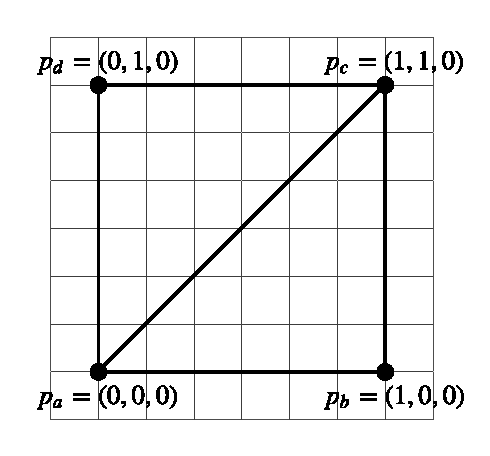
\includegraphics[width=\linewidth]{img/theory/Left-Interpolated.pdf}
    \caption{A plane in 3D space.}
    \label{fig:InterpolationLeft}
\end{subfigure}%
\begin{subfigure}{.5\textwidth}
    \centering
    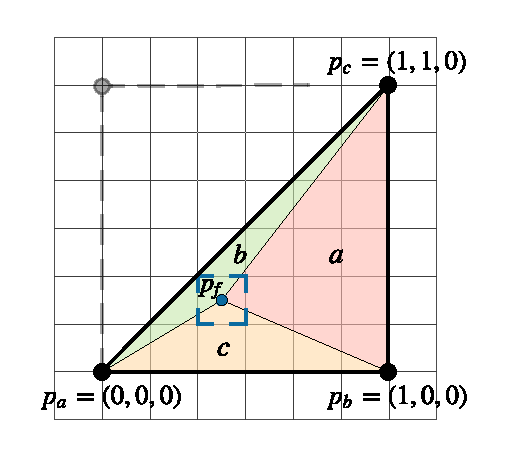
\includegraphics[width=\linewidth]{img/theory/Right-Interpolated.pdf}
    \caption{Interpolation of a triangle in the plane.}
    \label{fig:InterpolationRight}
\end{subfigure}
\caption{
    \textbf{(a)} Plane defined in 3D space made up of two triangles, with each vertex's \texttt{vert\_pos} attribute displayed. \textbf{(b)} After the rasterizer has decided which fragment belongs to which triangle, it's attributes (like \texttt{vert\_pos}) can be interpolated between the three vertices. The weights $a$, $b$ and $c$ are (more or less) equal to the inverse of the distances to their respective vertex.
}
\label{fig:Interpolation}
\end{figure}
An important thing to note is that by default convention, the pixel positions are located at \textit{half-pixel coordinates}, meaning that the actual coordinate for a pixel is the position of the center of that pixel \cite{segal_2013_the}. This does not matter much if the resolution is high, as the maximum error of the interpolated fragment position \codeinline[glsl]{frag_pos} we can get if we wrongly assume that the coordinates are given by the lower left corner of a pixel, is half a pixel, or $\frac{1}{r\cdot 2}$, where $r$ is the pixel resolution in some direction. Let $w$ and $h$ be the image width and height in pixels and $(x,y)$ the index of a pixel where $x \in [0,w-1], y \in [0,h-1]$. In general, a pixel's (or fragment's) position is given by equation \ref{eq:FragPos}. Because we need to model our shaders in Python as similar as possible to the OpenGL standard, this is something we must include when generating pixel positions, see section \ref{sec:RenderingInPython}.

\begin{equation}\label{eq:FragPos}
frag\_pos(x,y) = (x + \frac{x}{w \cdot 2}, y + \frac{y}{h \cdot 2}, 0)
\end{equation}


\section{Differentiable Rendering in DiPTeR}\label{sec:RenderingInDiPTeR}

\begin{enumerate}
    \item \st{Python rendering is only done in 2D}
    \item Have to implement the opengl standard library.
    \item The rendering itself is kept very simple, not taking any lighting or procedural 3D structures (bump maps etc) into account, as this thesis focuses on the generation and matching of procedural textures. 
\end{enumerate}

The python rendering should mimic the rendering process of OpenGL as closely as possible, so that a solution that's accurate for python will be accurate for OpenGL too. In our implementation of OpenGL, the vertex shader is essentially only used to interpolate vertex coordinates, so this step can be built in to our \codeinline{Shader} class as it only needs to be defined once. Each GLSL shader has an accompanying Python implementation; a subclass of our \codeinline{Shader} superclass and is required to implement the \codeinline{shade()}-function. This function has the same job as the fragment shader in that it takes the equivalent of GLSL function parameters as input, and returns a color for each fragment, or a fully rendered image in the matrix implementation, see section \ref{sec:MatrixImplementation}. Note that in our implementation, the rendered image matrix is column major, the standard for matrices representing images, but not for general tensor-like data structures in frameworks such as \textit{NumPy} and \textit{PyTorch}. We are also using 3 channels instead of 4, thus discarding the alpha value as it is difficult to account for opacity during inverse rendering. Furthermore, the Python rendering, by default, only renders to a 2D plane (z-coordinate is zero for all fragments), as its only job is to serve as a differentiable version of the OpenGL rendering pipeline for inverse rendering of 2D textures.

\subsection{Iterative implementation}\label{sec:IterativeImplementation}

This naive but simple implementation tries to model the way a fragment shader is called for each fragment (effectively pixel) independently and returns a color for that one fragment. The position of the fragment is given by the tensor \codeinline{vert_pos} on the form \codeinline{(x,y,z)} while \codeinline{**args} contains any optional parameters. To render an image, we first need to define its width and height in pixels and create an empty matrix of shape $(width, height, 3)$ to act as our image placeholder. As explained in section \ref{sec:Interpolation}, the positions of a pixel is given at center of each pixel, we need to generate their positions differently from the position in the matrix using \texttt{GetXs()} and \texttt{GetYs()} which emulate the interpolation of the \codeinline{frag_pos} variable that runs from $0$ to $1$. Then, each position in the matrix is assigned to the output of the render function, where we set the \codeinline{vert_pos} argument to the pixel position, and keep the other arguments constant. This algorithm is explained in pseudocode in \ref{alg:IterativeRendering}. 

\begin{algorithm}[H]
\SetKwData{Img}{img}\SetKwData{Width}{width}\SetKwData{Height}{height}\SetKwData{Xs}{xs}\SetKwData{Ys}{ys}\SetKwData{X}{x}\SetKwData{Y}{y}\SetKwData{FragPos}{frag\_pos}\SetKwData{Params}{params}
\SetKwFunction{Shade}{Shade}\SetKwFunction{GetXs}{GetXs}\SetKwFunction{GetYs}{GetYs}
\SetKwInOut{Input}{Input}\SetKwInOut{Output}{output}

\KwResult{A Tensor of size $w\times h \times 3$ containing the pixel data for the rendered image.}
\Input{A shade function \Shade and an image size (\Width, \Height).}

\BlankLine
Initialize \Img as empty matrix of size (\Width,\Height,3)\;
\Xs $\leftarrow$ \GetXs{\Width}\;
\Ys $\leftarrow$ \GetYs{\Height}\;
\For {\X $=0$ \KwTo \Width}{
    \For{\Y $=0$ \KwTo \Height}{
        set \FragPos $\leftarrow$ (\Xs{\X}, \Ys{\Y}, 0)\;
        Assign color at position (\X, \Y) of \Img to \Shade(\FragPos, \Params)\;
    }
}
\Return \Img\;
\caption{Iterative rendering algorithm}
\label{alg:IterativeRendering}
\end{algorithm}

While this implementation is straight forward and easily translated to and from GLSL, the two nested python for loops become a major performance bottleneck. All PyTorch functions are implemented and highly optimized in a C++ backend while Python for loops are notoriously slow. Furthermore, some shaders don't use the \codeinline{frag_pos} variable, and will thus have the same output for each pixel. Calling the shader function $width \times height$ times, when we could call it once and replicate the output over the entire image, is a huge waste of time. Another, even worse implication is the fact that PyTorch will add a node to the computational graph (see section \ref{sec:ComputationalGraph}) for each call to a PyTorch function. As such, this approach will add $width \times height$ duplicates to the node graph, making it much slower to traverse in the backward step as well as memory inefficient. Using only built in functions as far as possible can give a thousandfold performance boost, especially when rendering higher resolution images. How this is achieved is explained in the next section.

\subsection{Matrix implementation}\label{sec:MatrixImplementation}

\begin{enumerate}
    \item \st{Rendering can be sped up by only using matrix operations}
    \item \st{More difficult to think about, making tests more important}
    \item \st{Very difficult to achieve some effects with loops when counter is an argument}
    \item \st{Show a nice math matrix representation}
    \item \st{Makes the computational graph much simpler}
\end{enumerate}

Fortunately all PyTorch functions operate on Tensors, indifferent of the tensors' shape. Therefore, we can generate a matrix of the same size as the output image, but at each position in the matrix, the fragment position \codeinline{frag_pos} is stored as a list of $(x,y,z)$ coordinates. The output of the shader function is then an entire rendered image, and not only a pixel. Similarly, all the input arguments to the shader function are now matrices of the same dimension as the rendered image, so we are effectively providing the shader function with the parameter value at each pixel all at once.

\begin{equation}\label{eq:FragPosMatrix}
\begin{aligned}
    F[:,:,0] &= 
    \begin{bmatrix} 
        f_x(0,0)    & f_x(1,0)  & \dots     & f_x(w,0)  \\
        f_x(0,1)    & f_x(1,1)  & \dots     & f_x(w,1)  \\
        \vdots      & \vdots    & \ddots    & \vdots    \\
        f_x(0,h)    & f_x(1,h)  & \dots     & f_x(w,h)  
    \end{bmatrix} \\
    F[:,:,1] &= 
    \begin{bmatrix} 
        f_y(0,0)    & f_y(1,0)  & \dots     & f_y(w,0)  \\
        f_y(0,1)    & f_y(1,1)  & \dots     & f_y(w,1)  \\
        \vdots      & \vdots    & \ddots    & \vdots    \\
        f_y(0,h)    & f_y(1,h)  & \dots     & f_y(w,h)  
    \end{bmatrix} \\
    F[:,:,2] &= 
    \begin{bmatrix} 
        0    & 0  & \dots     & 0  \\
        0    & 0  & \dots     & 0  \\
        \vdots      & \vdots    & \ddots    & \vdots    \\
        0    & 0  & \dots     & 0  
    \end{bmatrix}
\end{aligned}
\end{equation}

Let $f(x,y)$ denote the function that generates the \codeinline{frag_pos}, as shown in equation \ref{eq:FragPos}, at each image integer index $(x,y)$, and let $f_x$, $f_y$, $f_z$ denote the $x$,$y$, and $z$ position returned by $f$, respectively. Equation \ref{eq:FragPosMatrix} shows the matrix $F$ that contains all the fragment positions, such that each position $i,j$ in the matrix contains the vector $f(i,j)$. As mentioned in section \ref{sec:IterativeImplementation} on the iterative version of this implementation, the potential performance boost is upwards thousands of times, depending on the shader function, as well as making the computational graph much simpler. However, moving all parameters from one dimension to two three dimensions does come with some implementational overhead as its slightly harder to translate shaders from GLSL to python, making tests more important. In many cases however, its simply a matter of expanding tensors to the correct size and being careful with indexing as all tensors contain its value for all positions in the image being rendered. An code comparison of this is shown in figure \ref{fig:IterativeMethodHSV} and \ref{fig:MatrixMethodHSV}, proving that most code can be kept almost identical. 

\begin{figure}[h]
    \begin{minted}{python}
def shade(self, frag_pos: Tensor, h: Tensor, s: Tensor, v: Tensor) -> Tensor:
    c = torch.tensor(6.0)
    K = torch.tensor((1.0, 2.0 / 3.0, 1.0 / 3.0, 3.0))
    K0 = torch.stack(K[0], K[0], K[0])
    
    p = torch.abs(gl.fract(torch.stack([h, h, h]) + K[0:3]) * c - \\
        torch.stack([K[3], K[3], K[3]]))
    color = v * gl.mix(K0, torch.clamp(p - K0, 0., 1.), s)
    return color
    \end{minted}
    
\caption{Python code for HSV shader using the iterative method. All Tensors are vectors.}
\label{fig:IterativeMethodHSV}
\end{figure}

\begin{figure}[h]
    \begin{minted}{python}
def shade_mat(self, h: Tensor, s: Tensor, v: Tensor) -> Tensor:
    Wi, He = Shader.width, Shader.height
    c = torch.tensor(6.0).repeat(Wi, He, 1)
    K = torch.tensor((1.0, 2.0 / 3.0, 1.0 / 3.0, 3.0)).repeat(Wi, He, 1)
    K0 = K[:, :, 0].unsqueeze(-1).repeat(1, 1, 3)
    
    p = torch.abs(gl.fract(h.repeat(1, 1, 3) + K[:, :, 0:3]) * c - \\
        K[:, :, 3].unsqueeze(-1).repeat(1, 1, 3))
    color = v * gl.mix(K0, torch.clamp(p - K0, 0., 1.), s)
    return color
    \end{minted}
    \caption{Python code for HSV shader using the matrix method. All Tensors are matrices, usually created using the PyTorch \codeinline{repeat()} function that repeats a tensor any number of times along specified dimensions. The PyTorch function \codeinline{unsqueeze()} is sometimes needed to add a dimension to tensors. Additionally, the \codeinline{frag_pos} argument, not used here, no longer needs to be passed to the shade function, instead one copy is generated and saved as an attribute in the \codeinline{Shader} class.}
    \label{fig:MatrixMethodHSV}
\end{figure}

There does, however, exist a truly limiting drawback to the matrix method when it comes to loops, where the loop count is dictated by an argument to the shader function. As mentioned, all arguments are matrices, and there exists no implementation of a function that can map a function over values of a Tensor in PyTorch. Consider the code example in figure \ref{fig:MatrixMethodForProblem} with a shade function that takes one parameter \codeinline{D} as input, where \codeinline{f()} is any arbitrary function. If \codeinline{D} in this example is an integer scalar, we would not have a problem, but in our matrix implementation, it is a matrix tensor of shape \codeinline{(w,h,1)}, meaning each pixel could potentially have different values. Without a function to map other functions to each element in a matrix, this is very difficult to solve.

\begin{figure}
    \centering
    \begin{minted}{python}
def shade(self, D: Tensor):
    w, h = Shader.width, Shader.height
    v = torch.tensor(0.0).repeat(w,h,1)
    a = torch.tensor(0.5).repeat(w,h,1)

    for t in range(D):
        v = v + f(a)
        a = a * 0.5
        
    return v
    \end{minted}
    \caption{An example of a shader that is very difficult to translate to our matrix form, as \codeinline{D} is a matrix with a potentially different value for each pixel, while in an iterative method, the \codeinline{shade()} function would be executed for each pixel, and \codeinline{D} would simply be an integer scalar tensor.}
    \label{fig:MatrixMethodForProblem}
\end{figure}

\subsection{Testing shader implementation likeness}

\begin{enumerate}
    \item We need to ensure that our implementations generate the same results.
    \item Explain the minimum MSE error we can expect.
\end{enumerate}

\section{Composite Shaders}\label{sec:CompositeShaders}
\begin{enumerate}
    \item How is it done in GLSL (recompiling the code)?
    \item "had to" implement preprocessing like "\#import"
    \item Talk about only one main function, the rest is implemented as simply functions.
    \item How is it done in python, how are Tensors tracked and returned so that the same reference is always returned for \texttt{render()}, otherwise backprop will not work...
    \item Explain that this is possible due to PyTorch only tracking torch operations done on it.
\end{enumerate}

\subsection{\texttt{\#import} Preprocessor Directive}\label{sec:ImportPreprocessorDirective}




\section{Node Editor}

\begin{enumerate}
    \item Maybe show a simple UML over the code design
\end{enumerate}

\section{Inverse Rendering}

\begin{enumerate}
    \item Gradient Descent implementation
    \item Different Optimizers
    \item Forward mainly uses GLSL while backward uses python implementation...
    \item every iteration the updated render is shown for both python and GLSL with new parametrs...
    \item loss is plotted...
\end{enumerate}


